\documentclass[a4paper]{article}
\usepackage{vntex}
%\usepackage[english,vietnam]{babel}
%\usepackage[utf8]{inputenc}

%\usepackage[utf8]{inputenc}
%\usepackage[francais]{babel}
\usepackage{a4wide,amssymb,epsfig,latexsym,multicol,array,hhline,fancyhdr}
\usepackage{booktabs}
\usepackage{amsmath}
\usepackage{lastpage}
\usepackage[lined,boxed,commentsnumbered]{algorithm2e}
\usepackage{enumerate}
\usepackage{color}
\usepackage{graphicx}							% Standard graphics package
\usepackage{float}
\usepackage{array}
\usepackage{tabularx, caption}
\usepackage{multirow}
\usepackage[framemethod=tikz]{mdframed}% For highlighting paragraph backgrounds
\usepackage{multicol}
\usepackage{rotating}
\usepackage{graphics}
\usepackage{geometry}
\usepackage{setspace}
\usepackage{epsfig}
\usepackage{tikz}
\usepackage{listings}
\usetikzlibrary{arrows,snakes,backgrounds}
\usepackage{hyperref}
\hypersetup{urlcolor=blue,linkcolor=black,citecolor=black,colorlinks=true} 
%\usepackage{pstcol} 								% PSTricks with the standard color package

\newtheorem{theorem}{{\bf Định lý}}
\newtheorem{property}{{\bf Tính chất}}
\newtheorem{proposition}{{\bf Mệnh đề}}
\newtheorem{corollary}[proposition]{{\bf Hệ quả}}
\newtheorem{lemma}[proposition]{{\bf Bổ đề}}

\everymath{\color{blue}}
%\usepackage{fancyhdr}
\setlength{\headheight}{40pt}
\pagestyle{fancy}
\fancyhead{} % clear all header fields
\fancyhead[L]{
 \begin{tabular}{rl}
    \begin{picture}(25,15)(0,0)
    \put(0,-8){
\includegraphics[width=8mm, height=8mm]{logoITSGUsmall.png}}
    %\put(0,-8){\epsfig{width=10mm,figure=hcmut.eps}}
   \end{picture}&
	%\includegraphics[width=8mm, height=8mm]{hcmut.png} & %
	\begin{tabular}{l}
		\textbf{\bf \ttfamily Trường Đại học Sài Gòn}\\
		\textbf{\bf \ttfamily Khoa Công Nghệ Thông Tin}
	\end{tabular} 	
 \end{tabular}
}
\fancyhead[R]{
	\begin{tabular}{l}
		\tiny \bf \\
		\tiny \bf 
	\end{tabular}  }
\fancyfoot{} % clear all footer fields
\fancyfoot[L]{\scriptsize \ttfamily Bài tập lớn môn Phát triển phần mềm mã nguồn mở - Niên khóa 2024-2025}
\fancyfoot[R]{\scriptsize \ttfamily Trang {\thepage}/\pageref{LastPage}}
\renewcommand{\headrulewidth}{0.3pt}
\renewcommand{\footrulewidth}{0.3pt}


%%%
\setcounter{secnumdepth}{4}
\setcounter{tocdepth}{3}
\makeatletter
\newcounter {subsubsubsection}[subsubsection]
\renewcommand\thesubsubsubsection{\thesubsubsection .\@alph\c@subsubsubsection}
\newcommand\subsubsubsection{\@startsection{subsubsubsection}{4}{\z@}%
                                     {-3.25ex\@plus -1ex \@minus -.2ex}%
                                     {1.5ex \@plus .2ex}%
                                     {\normalfont\normalsize\bfseries}}
\newcommand*\l@subsubsubsection{\@dottedtocline{3}{10.0em}{4.1em}}
\newcommand*{\subsubsubsectionmark}[1]{}
\makeatother

\definecolor{dkgreen}{rgb}{0,0.6,0}
\definecolor{gray}{rgb}{0.5,0.5,0.5}
\definecolor{mauve}{rgb}{0.58,0,0.82}

\lstset{frame=tb,
	language=Matlab,
	aboveskip=3mm,
	belowskip=3mm,
	showstringspaces=false,
	columns=flexible,
	basicstyle={\small\ttfamily},
	numbers=none,
	numberstyle=\tiny\color{gray},
	keywordstyle=\color{blue},
	commentstyle=\color{dkgreen},
	stringstyle=\color{mauve},
	breaklines=true,
	breakatwhitespace=true,
	tabsize=3,
	numbers=left,
	stepnumber=1,
	numbersep=1pt,    
	firstnumber=1,
	numberfirstline=true
}

\begin{document}

\begin{titlepage}
\begin{center}
TRƯỜNG ĐẠI HỌC SÀI GÒN \\
KHOA CÔNG NGHỆ THÔNG TIN
\end{center}
\vspace{1cm}

\begin{figure}[h!]
\begin{center}

\includegraphics[width=3cm]{logoITSGU.png}
\end{center}
\end{figure}

\vspace{1cm}


\begin{center}
\begin{tabular}{c}
	\multicolumn{1}{l}{\textbf{{\Large Phát triển phần mềm mã nguồn mở}}}\\
	~~\\
	\hline
	\\
	\multicolumn{1}{l}{\textbf{{\Large  }}}\\
	\\
	
	\textbf{{\Huge Phát triển phần mềm Spotify Clone}}\\
	\\
	\hline
\end{tabular}
\end{center}

\vspace{3cm}

\begin{table}[h]
\begin{tabular}{rrl}
\hspace{5 cm} & GVHD: &Từ Lãng Phiêu\\
& SV: & Bùi Công Thạch - 3121410445\\
& & Cao Huy Hưng - 3121410237 \\
& & Bùi Công Tuấn - 3121410553 \\
\end{tabular}
\vspace{1 cm}
\end{table}

\begin{center}
    {\footnotesize Email liên hệ nhóm: buithach.it@gmail.com}
\end{center}
\vspace{1 cm}
\begin{center}

{\footnotesize TP. HỒ CHÍ MINH, THÁNG 5/2025}
\end{center}
\end{titlepage}


\thispagestyle{empty}

\newpage

\begin{center}
    {\Large \textbf{NHẬN XÉT CỦA GIẢNG VIÊN}}
\end{center}

\newpage

\newpage
\begin{center}
    \textbf{{\Huge LỜI CẢM ƠN}}
\end{center}

Trước hết, nhóm chúng em xin gửi lời cảm ơn chân thành đến Trường Đại học Sài Gòn, Khoa Công nghệ Thông tin đã tạo điều kiện để chúng em thực hiện tiểu luận này.\\

Chúng em xin bày tỏ lòng biết ơn sâu sắc đến giảng viên hướng dẫn, người đã tận tình hỗ trợ, định hướng và góp ý để chúng em có thể hoàn thiện đề tài này.\\

Bên cạnh đó, chúng em cũng xin gửi lời cảm ơn đến các doanh nghiệp, chuyên gia đã chia sẻ thông tin, kinh nghiệm thực tế, giúp chúng em có cái nhìn rõ hơn về việc phát triển phần mềm mã nguồn mở. Cuối cùng, chúng em xin cảm ơn gia đình, bạn bè đã luôn động viên, hỗ trợ trong suốt quá trình thực hiện đề tài này.\\

Nhóm chúng em rất mong nhận được ý kiến đóng góp để hoàn thiện hơn nữa nghiên cứu này.

\newpage

\newpage
\begin{center}
    \textbf{{\Huge LỜI MỞ ĐẦU}}
\end{center}

Trong thời đại công nghệ số phát triển không ngừng, các ứng dụng phát nhạc trực tuyến đã trở thành một phần quen thuộc trong đời sống giải trí của con người. Spotify – một trong những nền tảng phát nhạc phổ biến nhất hiện nay – không chỉ thu hút người dùng bởi kho nhạc phong phú mà còn bởi giao diện hiện đại và trải nghiệm người dùng thân thiện. Từ đó, nhóm chúng em đã chọn thực hiện đề tài Spotify Clone như một cách học hỏi và rèn luyện kỹ năng xây dựng ứng dụng thực tế.\\

Trong quá trình thực hiện, nhóm đã có cơ hội tiếp cận và ứng dụng các công nghệ mã nguồn mở như React, TypeScript, Django và GitHub. Đề tài được triển khai theo mô hình SPA, kết hợp giữa frontend, backend và WebSocket, giúp nhóm hiểu rõ hơn về cách các thành phần trong hệ thống tương tác với nhau. Các tính năng như phát nhạc, tìm kiếm, quản lý danh sách phát và trò chuyện thời gian thực đã được tích hợp nhằm tái hiện một phần trải nghiệm thực tế từ Spotify.\\

Thông qua đồ án này, nhóm không chỉ củng cố kiến thức đã học mà còn nâng cao kỹ năng làm việc nhóm, quản lý tiến độ dự án, tìm hiểu công nghệ mới và giải quyết các vấn đề phát sinh trong quá trình phát triển phần mềm.\\

Chúng em xin chân thành cảm ơn thầy đã tạo điều kiện để nhóm thực hiện đề tài này. Mặc dù đã cố gắng hoàn thiện trong khả năng của mình, đồ án vẫn không tránh khỏi những thiếu sót. Nhóm rất mong nhận được sự góp ý để cải thiện tốt hơn trong tương lai.

\newpage

%%%%%%%%%%%%%%%%%%%%%%%%%%%%%%%%%

%%%%%%%%%%%%%%%%%%%%%%%%%%%%%%%%%


\newpage
\tableofcontents
\newpage

%%%%%%%%%%%%%%%%%%%%%%%%%%%%%%%%%


%%%%%%%%%%%%%%%%%%%%%%%%%%%%%%%%%
\section{Giới thiệu đề tài}
\subsection{Giới thiệu Spotify Clone}
		\textbf
		Spotify Clone là một ứng dụng nghe nhạc trực tuyến được xây dựng với mục tiêu mô phỏng lại giao diện và chức năng cơ bản của Spotify – nền tảng phát nhạc trực tuyến nổi tiếng toàn cầu. Ứng dụng cho phép người dùng nghe nhạc, xem danh sách bài hát, tìm kiếm bài hát và phát bài hát theo thời gian thực với trải nghiệm thân thiện. Dự án này được phát triển theo mô hình SPA (Single Page Application) sử dụng Angular ở phía frontend, Django ở phía backend và WebSocket cho việc xử lý dữ liệu thời gian thực.
	\subsection{Lý do chọn đề tài}
    
	\textbf{Lý do chọn đề tài}
	Trong thời đại công nghệ số phát triển mạnh mẽ, nhu cầu nghe nhạc trực tuyến ngày càng trở nên phổ biến và thiết yếu trong đời sống hằng ngày. Các nền tảng như Spotify không chỉ đơn thuần là công cụ giải trí mà còn trở thành một phần trong thói quen và phong cách sống của người dùng hiện đại. Tuy nhiên, để xây dựng một ứng dụng nghe nhạc trực tuyến chuyên nghiệp, hiện đại và có tính tương tác cao như Spotify đòi hỏi nhiều kiến thức liên quan đến lập trình giao diện, xử lý âm thanh, quản lý cơ sở dữ liệu và tối ưu hiệu năng.

Vì vậy, em chọn đề tài Spotify Clone với mục tiêu:

    Tìm hiểu và thực hành quy trình xây dựng một ứng dụng nghe nhạc từ đầu đến cuối.

    Áp dụng các kiến thức về phát triển phần mềm như UI/UX, kết nối backend, quản lý media và phát triển tính năng tương tác người dùng.

    Rèn luyện khả năng thiết kế hệ thống phần mềm có cấu trúc rõ ràng, dễ mở rộng và nâng cấp trong tương lai.

Đề tài không chỉ mang tính thực tiễn cao mà còn giúp em phát triển kỹ năng tư duy hệ thống, làm việc với công nghệ hiện đại và chuẩn bị nền tảng tốt cho các dự án phần mềm quy mô lớn hơn sau này.
    \subsection{Mục tiêu}
    \textbf
    Thiết kế giao diện web phần mềm Spotify Clone và lập trình bằng ngôn ngữ Python.\\
    Front end: React hoặc Angular\\
    Backend: Django\\
    Database:MySql\\
    Các tính năng cơ bản cho ứng dụng sử dụng trên mã nguồn mở Linux.
    Yêu cầu phát triển phần mềm Spotify Clone:\\
    1. Chức năng phát nhạc:\\
    2. Chức năng phát video âm nhạc:\\
    3. Chức năng tải video âm nhạc:\\
    4. Chức năng User tạo abum, bài hát yêu thích\\
    5. Trang Admin.\\
    6. Optional: Có thêm tính năng chat tích hợp trong giao diện web
spotify clone.\\
    \subsection{Đối tượng và phạm vi sử dụng}
    \textbf
    Đối tượng sử dụng: người dùng cá nhân, sinh viên, lập trình viên học tập và trải nghiệm giao diện nghe nhạc hiện đại.\\
    Phạm vi: ứng dụng chủ yếu tập trung vào frontend với một số chức năng backend mô phỏng như phát nhạc, danh sách bài hát và xử lý trạng thái phát. Chưa tích hợp thanh toán, tải bài hát, đề xuất AI hoặc tính năng bảo mật cao.



\section{{CÔNG NGHỆ VÀ PHẦN MỀM MÃ NGUỒN MỞ SỬ DỤNG}}
    \subsection{Tổng quan dự án}
    \textbf{}
    Dự án Spotify Clone là một ứng dụng web mô phỏng các chức năng chính của Spotify, bao gồm phát nhạc, quản lý playlist, tìm kiếm bài hát và phân quyền người dùng. Ứng dụng được xây dựng với:
    
    Frontend: React (TypeScript), Tailwind CSS, Ant Design
    
    Backend: Django REST Framework, MySQL, JWT Authentication
    \subsection{Kiến trúc Frontend}
    \textbf{Công nghệ sử dụng:}\\
    \begin{itemize}
        \item React : Thư viện JavaScript để xây dựng giao diện người dùng.
        \item TypeScript: Ngôn ngữ lập trình mở rộng của JavaScript, cung cấp kiểu dữ liệu tĩnh.
        \item Tailwind CSS: Framework CSS tiện ích-first để thiết kế giao diện nhanh chóng.
        \item Vite: Công cụ build nhanh chóng cho các dự án frontend.
        \item React Router DOM: Thư viện định tuyến cho React.
        \item Axios: Thư viện HTTP client để giao tiếp với backend.
        \item Ant Design: Thư viện UI component cho React.
        \item React Spinners: Thư viện spinner cho trạng thái loading.
        \item SimpleBar React: Thư viện thanh cuộn tùy chỉnh cho React.
    \end{itemize}
    \textbf{Tính năng chính:}\\
    \begin{itemize}
        \item Xác thực người dùng: Đăng nhập/Đăng ký với JWT.
        \item Phát nhạc: Điều khiển play/pause, next/previous.
        \item Quản lý playlist: Tạo, chỉnh sửa, xóa playlist.
        \item Tìm kiếm bài hát: Tìm kiếm theo tên bài hát hoặc nghệ sĩ.
        \item Điều chỉnh âm lượng: Tăng/giảm âm lượng phát nhạc.
        \item Chế độ Shuffle và Repeat: Phát ngẫu nhiên hoặc lặp lại bài hát.
        \item Phân quyền người dùng: Quản trị viên (superuser) có quyền quản lý nội dung.
    \end{itemize}

\subsection{Kiến trúc Backend}
    \textbf{Công nghệ sử dụng:}
    \begin{itemize}
        \item Django: Framework web mạnh mẽ cho Python.
        \item Django REST Framework: Thư viện xây dựng API RESTful.
        \item MySQL: Hệ quản trị cơ sở dữ liệu quan hệ.
        \item JWT Authentication: Xác thực người dùng bằng JSON Web Token.
        \item CORS Headers: Xử lý Cross-Origin Resource Sharing cho API.
    \end{itemize}
    \textbf{Tính năng chính:}
    \begin{itemize}
        \item API RESTful: Cung cấp các endpoint cho frontend tương tác.
        \item Xác thực và phân quyền: Sử dụng JWT để xác thực và phân quyền người dùng.
        \item Quản lý dữ liệu: CRUD cho người dùng, bài hát, playlist.
        \item Bảo vệ bản quyền: Đảm bảo chỉ người dùng có quyền mới truy cập được nội dung.
    \end{itemize}

    \subsection{Tính năng chat}
    Đối tượng chat:
    Người dùng sẽ chat với một hệ thống AI (không phải người thật).\\
    Cụ thể, backend sử dụng mô hình AI (Google GenAI (Gemini 2.0 Flash)) để:\\
    \begin{enumerate}
        \item Nhận câu hỏi tự nhiên từ người dùng (ví dụ: "Các bài hát trong album Vol 1 là gì?").
        \item Sinh ra câu lệnh SQL phù hợp với câu hỏi đó.
        \item Thực thi SQL trên cơ sở dữ liệu nhạc (tracks, albums, artists).
        \item Trả về kết quả và sinh ra câu trả lời tự nhiên, lịch sự, bằng tiếng Việt cho người dùng.
    \end{enumerate}
    Luồng xử lý:
        \begin{itemize}
            \item Người dùng gửi câu hỏi qua API /chatbox/.
            \item Backend dùng AI để chuyển đổi câu hỏi thành SQL, truy vấn dữ liệu, rồi lại dùng AI để trả lời tự nhiên dựa trên kết quả truy vấn.
            \item Người dùng nhận được câu trả lời như đang trò chuyện với một trợ lý ảo am hiểu về nhạc.
        \end{itemize}

 \section{PHÂN TÍCH VÀ THIẾT KẾ SPOTIFY CLONE}
    \subsection{Mô hình ứng dụng}
    \textbf{Kiến trúc tổng quan}\\
    \\
    Ứng dụng được xây dựng theo mô hình client-server:
    
    \begin{itemize}
        \item Frontend: React (Vite, TypeScript, Ant Design)\\
        Giao diện người dùng, routing, gọi API, quản lý state, bảo vệ route, hiển thị dữ liệu nhạc, quản trị, xác thực...
        \item Backend: Python Django\\
        Xử lý logic nghiệp vụ, quản lý dữ liệu (users, tracks, albums, playlists, chatbox...), cung cấp API RESTful, tích hợp AI Gemini cho chat thông minh.
        \item Database: MySQL\\
        Lưu trữ dữ liệu nhạc, người dùng, playlist, v.v.
    \end{itemize}
    \textbf{Giao tiếp:}
    \begin{itemize}
        \item Frontend gọi API của backend qua HTTP (REST API).
        \item Backend xử lý, truy vấn database, trả kết quả về frontend.
    \end{itemize}

    
    \subsection{Các tính năng được xây dựng}
    \begin{itemize}
        \item Tìm kiếm, nghe nhạc, xem thông tin nghệ sĩ, album, playlist.
        \item Đăng ký, đăng nhập, phân quyền user/admin.
        \item Quản trị hệ thống (admin): Quản lý users, tracks, artists.
        \item Chat thông minh với AI Gemini: Hỏi đáp về nhạc, album, ca sĩ.
        \item Giao diện hiện đại, responsive, trải nghiệm người dùng tốt.
        \item Bảo vệ route, xác thực, phân quyền chặt chẽ.
    \end{itemize}

    \subsection{Xây dựng Database}
    \textbf{Xây dựng Cơ sở dữ liệu theo mô hình:}
    
\begin{figure}[H]
    \centering
    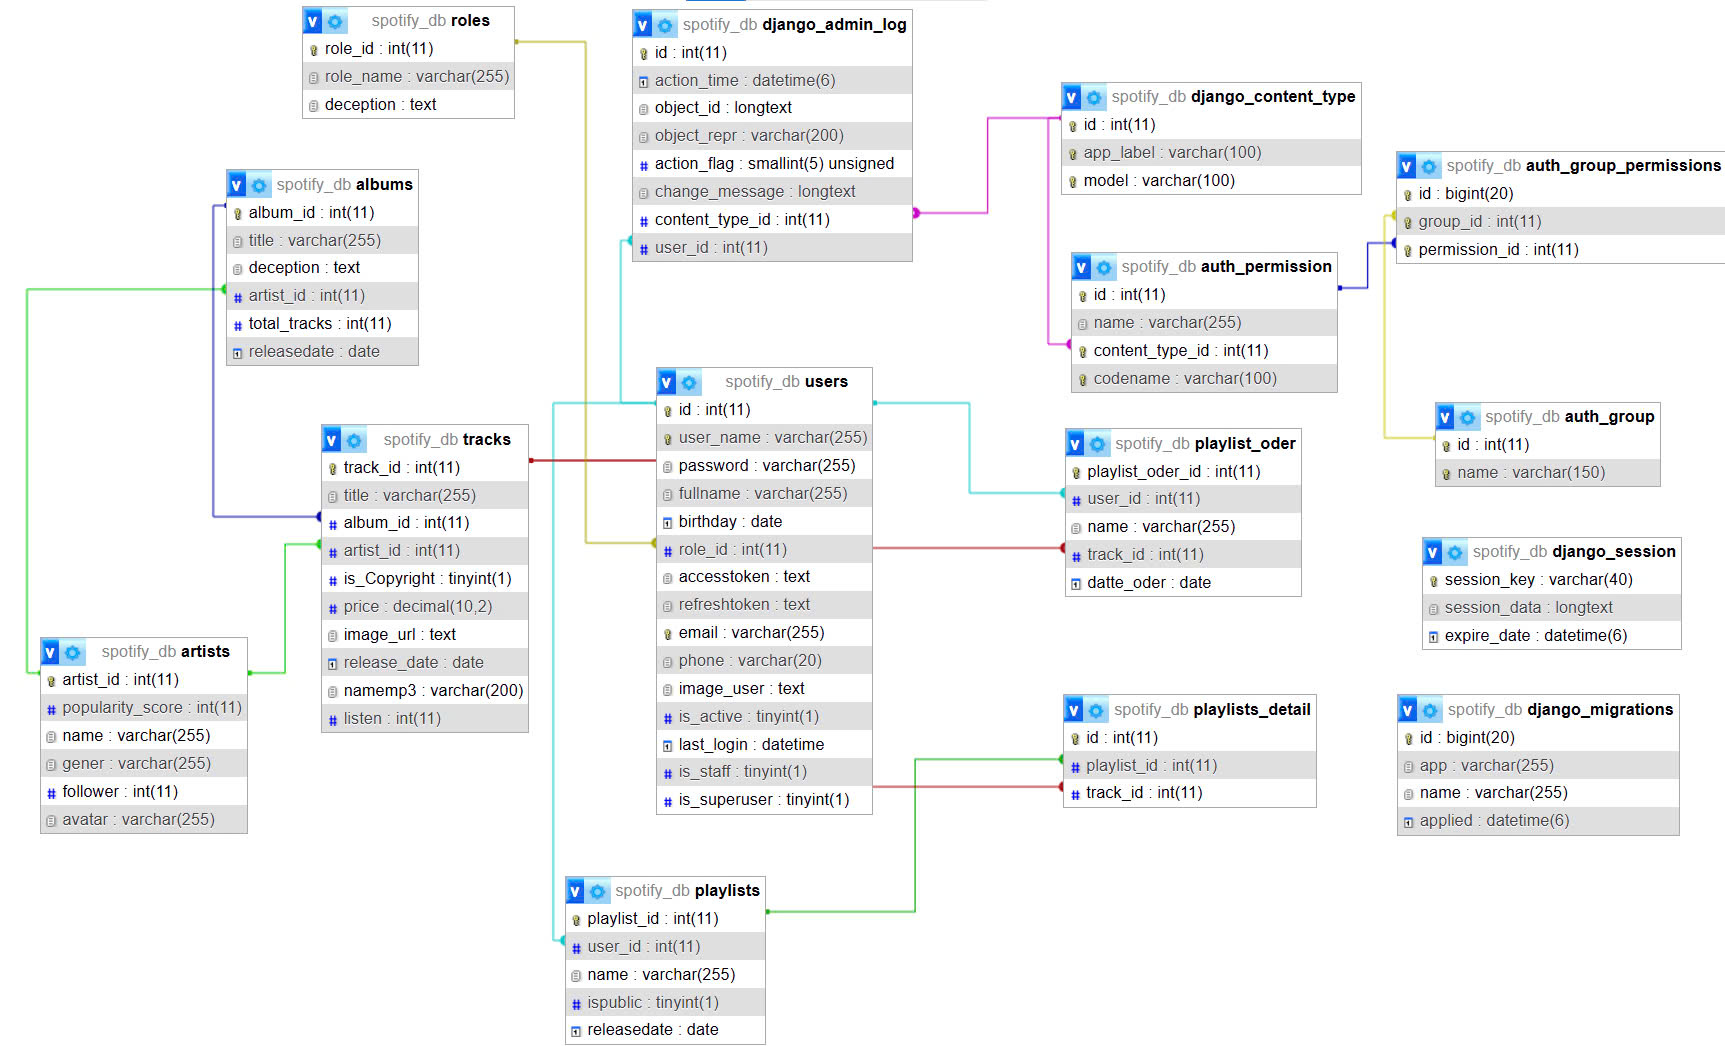
\includegraphics[width=1\linewidth]{img/database.jpg}
    \label{fig:enter-label}
\end{figure}
    
    \section{CÁCH CÀI ĐẶT ỨNG DỤNG}
    \subsection{Yêu cầu hệ thống}
    \textbf{Node.js (v14 trở lên)\\
    Python (v3.8 trở lên)\\
    MySQL}
    
    \subsection{Frontend}
    \begin{mdframed}
        [hidealllines=true,backgroundcolor=magenta!10]
		\begin{lstlisting}
        % Di chuyen Vao thu muc frontend %
        cd du-an-fontend-react/spotifyFrontEndProject
        
        % Cai det dependencies %
        npm install
        
        % Chay development server %
        npm run dev
        \end{lstlisting}
    \end{mdframed}

    \subsection{Backend}
        \begin{mdframed}
        [hidealllines=true,backgroundcolor=magenta!10]
		\begin{lstlisting}
        % Di chuyen vao thu muc backend %
        cd du-an-backend-python-django-be 
        
        % Tao moi truong ao %
        python -m venv venv
        
        % Kich hoat moi truong ao %
        % Windows
        venv\Scripts\activate
        % Linux/Mac %
        source venv/bin/activate
        
        % Cai dat dependencies %
        pip install -r requirements.txt
        
        % Chay migrations %
        python manage.py migrate
        
        % Chay development server %
        python manage.py runserver
        \end{lstlisting}
    \end{mdframed}

 \section{CẤU TRÚC VÀ MÔ HÌNH}
    \subsection{Cấu trúc thư mục của Project}
\begin{figure}[h!]
\begin{center}
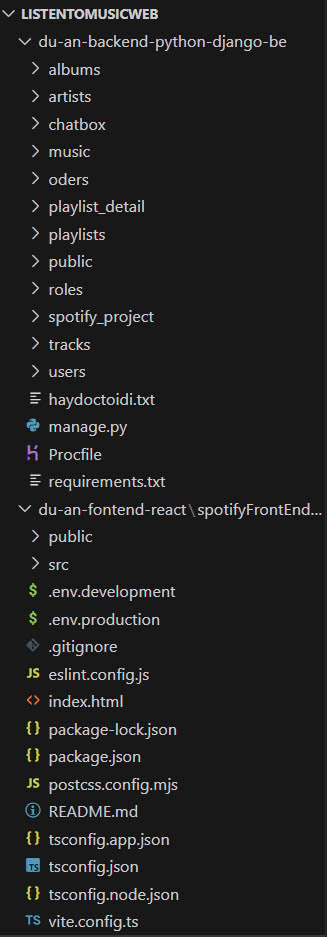
\includegraphics[width=6cm]{img/thumuc1.jpg}
\end{center}
\end{figure}

\newpage

    \subsection{Thư mục Backend}
    Đây là phần phía máy chủ (server), sử dụng Django – một framework Python mạnh mẽ để xây dựng API, xử lý dữ liệu, xác thực người dùng và giao tiếp với cơ sở dữ liệu. Dựa vào cấu trúc, có thể thấy mỗi thư mục con bên trong là một Django App, đại diện cho từng chức năng riêng biệt:\\

    \vspace{0.5cm}
    \begin{table}[h]
        \centering
        \begin{tabular}{|l|l|} \hline 
             Tên thư mục& Mô tả chức năng\\ \hline 
             albums/
& Quản lý thông tin các album âm nhạc\\ \hline 
             artists/& Quản lý thông tin nghệ sĩ\\ \hline 
             tracks/& Quản lý các bài hát (track)\\ \hline 
             users/& Quản lý tài khoản, thông tin người dùng\\ \hline 
             roles/& Quản lý vai trò, phân quyền người dùng
\\ \hline 
             playlists/; playlistdetail/ & 
Quản lý danh sách phát nhạc\\ \hline 
 chatbox/&Xử lý tính năng trò chuyện\\\hline
             manage.py& Tập tin chính để khởi chạy và quản lý dự án Django\\ \hline
        \end{tabular}
\caption{Thư mục Backend}
        \label{tab:my_label}
    \end{table}

    Mỗi app sẽ có các tệp chuẩn như:
\begin{itemize}
    \item models.py: định nghĩa bảng dữ liệu (model).
    \item views.py: viết các xử lý logic.
    \item urls.py: định nghĩa các API endpoint riêng cho app.
    \item serializers.py: chuyển đổi dữ liệu từ model sang JSON (nếu dùng Django REST Framework).
\end{itemize}

\subsection{Thư mục Frontend}
Đây là dự án frontend chính, được xây dựng bằng React và TypeScript, sử dụng Vite làm công cụ build. Dự án này có cấu trúc thư mục rõ ràng, bao gồm các thư mục như src/ (chứa code chính), public/ (tài nguyên tĩnh), và các file cấu hình như package.json, tsconfig.json, vite.config.ts, v.v. 

\begin{table}[h]
    \centering
    \begin{tabular}{|l|l|} \hline 
         Tên thư mục& Mô tả chức năng\\ \hline
         components/& Xây dựng UI, chia nhỏ theo chức năng.\\ \hline 
         pages/& Các trang chính, routing.\\ \hline 
         services/& Xử lý logic, gọi API.\\ \hline
         styles/&Quản lý style chung.\\\hline
         types/&Định nghĩa kiểu dữ liệu.\\\hline
    \end{tabular}
    \caption{Thư mục Frontend}
    \label{tab:my_label}
\end{table}

Cấu trúc thư mục src/ được tổ chức hợp lý, mỗi phần như pages, components, services, types,... đều đảm nhận một vai trò riêng biệt, giúp mã nguồn rõ ràng, dễ bảo trì và mở rộng.\\
\\
Thư mục pages/\\
\begin{itemize}
    \item Chứa các trang chính của ứng dụng, mỗi trang (ví dụ: home, search, playlist, artist, login, register,...) được tách thành các file/module riêng biệt. Điều này giúp dễ dàng quản lý routing, tối ưu hiệu suất khi chỉ tải những phần cần thiết cho người dùng truy cập từng trang.
\end{itemize}
Thư mục services/\\
\begin{itemize}
    \item Tập trung toàn bộ các logic giao tiếp với API (backend), ví dụ như cấu hình axios, các hàm gọi API. Việc này giúp mã nguồn tách biệt rõ ràng giữa phần giao diện và phần xử lý dữ liệu, dễ kiểm thử và tuân thủ nguyên tắc Separation of Concerns (SoC).
\end{itemize}
Thư mục components/
\begin{itemize}
    \item Chứa các component tái sử dụng như layout, header, navbar, footer, các thành phần giao diện nhỏ,... Việc gom nhóm này giúp đảm bảo tính đồng nhất giao diện, tiết kiệm công sức khi phát triển hoặc thay đổi layout sau này.
\end{itemize}
Thư mục styles/
\begin{itemize}
    \item Quản lý các file style chung (CSS/SCSS), giúp dễ dàng tùy biến giao diện toàn ứng dụng và tái sử dụng các biến, mixin, style toàn cục.
\end{itemize}
Thư mục types/
\begin{itemize}
    \item Định nghĩa các kiểu dữ liệu dùng chung cho toàn dự án, giúp tăng tính an toàn khi lập trình với TypeScript, giảm lỗi khi truyền dữ liệu giữa các thành phần.
\end{itemize}

\subsection{Routing và phân chia các module}
Dự án được tổ chức theo kiến trúc module hóa, tức là chia nhỏ hệ thống thành các phần riêng biệt tương ứng với từng chức năng cụ thể. Việc phân chia này được áp dụng ở cả hai phía: Backend (Django) và Frontend (Angular), nhằm tăng tính mở rộng, dễ bảo trì và giúp các thành viên trong nhóm có thể phát triển song song mà không ảnh hưởng đến nhau.\\
\\
\textbf{Backend (Django)}\\
\\
Phía backend được xây dựng bằng framework Django, mỗi chức năng được tổ chức dưới dạng một app riêng biệt. Ví dụ: albums, artists, tracks, users, chat,... Mỗi app đóng vai trò như một module độc lập, đảm nhiệm một phần nghiệp vụ của hệ thống như quản lý bài hát, người dùng, hoặc trò chuyện.\\
\\
Mỗi app sẽ có các file riêng như:\\
\begin{itemize}
    \item models.py: định nghĩa bảng dữ liệu
    \item views.py: xử lý logic nghiệp vụ
    \item urls.py: định tuyến API cho từng app
\end{itemize}
Tất cả các tuyến đường (route) của các app sẽ được gom lại trong file backend/urls.py chính bằng cách sử dụng hàm include(), giúp dự án dễ tổ chức và mở rộng.\\

\begin{figure}[H]
    \centering
    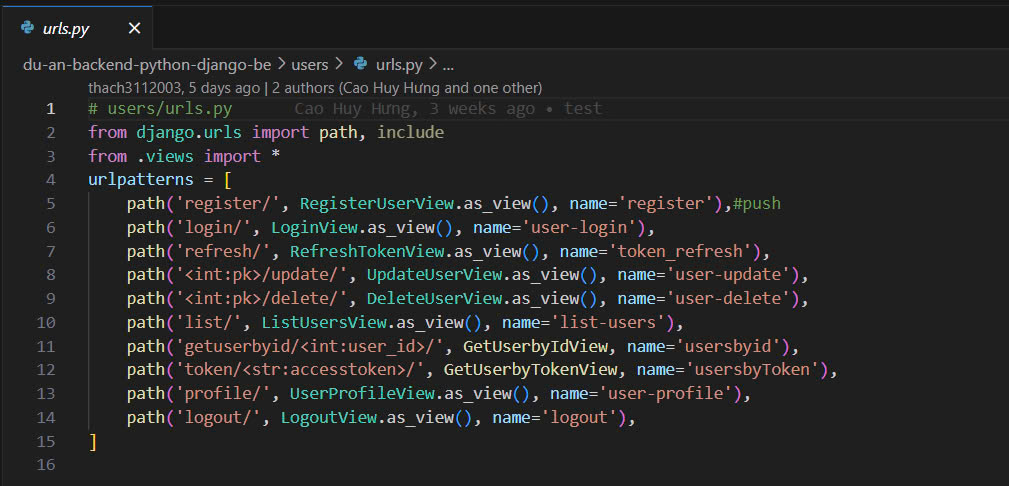
\includegraphics[width=0.9\linewidth]{img/userUrls.jpg}
    \label{fig:enter-label}
\end{figure}

Nhờ đó, khi frontend gọi các API như GET : 	/users/list/ , Django sẽ biết được phải định tuyến đến app users\\
\\
\\
\textbf{Frontend (React)}\\
Ứng dụng sử dụng thư viện react-router-dom để quản lý routing.\\
Tất cả các route được khai báo tập trung trong file src/main.tsx thông qua createBrowserRouter.

\textbf{Routing (Định tuyến)}
\\Phân chia route chính:
\\
\\ Người dùng thông thường:
\begin{itemize}
    \item / → Trang chủ (HomePage)
    \item /search → Trang tìm kiếm (SearchPage)
    \item /playlist/:playlistId/:playlistName → Trang chi tiết playlist
    \item /artist/:artistId/:artistName → Trang nghệ sĩ
    \item /login, /register → Đăng nhập, đăng ký
    \\
    \\ Trang đặc biệt:
    \item /checkout → Trang thanh toán (yêu cầu đăng nhập, dùng ProtectedRoute)\\
    \\
    Quản trị (Admin):
    \item /admin → Layout quản trị (yêu cầu đăng nhập, dùng ProtectedRoute)
    \item /admin/user → Quản lý người dùng
    \item /admin/track → Quản lý bài hát
    \item /admin/singer → Quản lý ca sĩ
\end{itemize}

\begin{figure}[H]
  \centering
  \begin{minipage}[b]{0.52\textwidth}
    \centering
    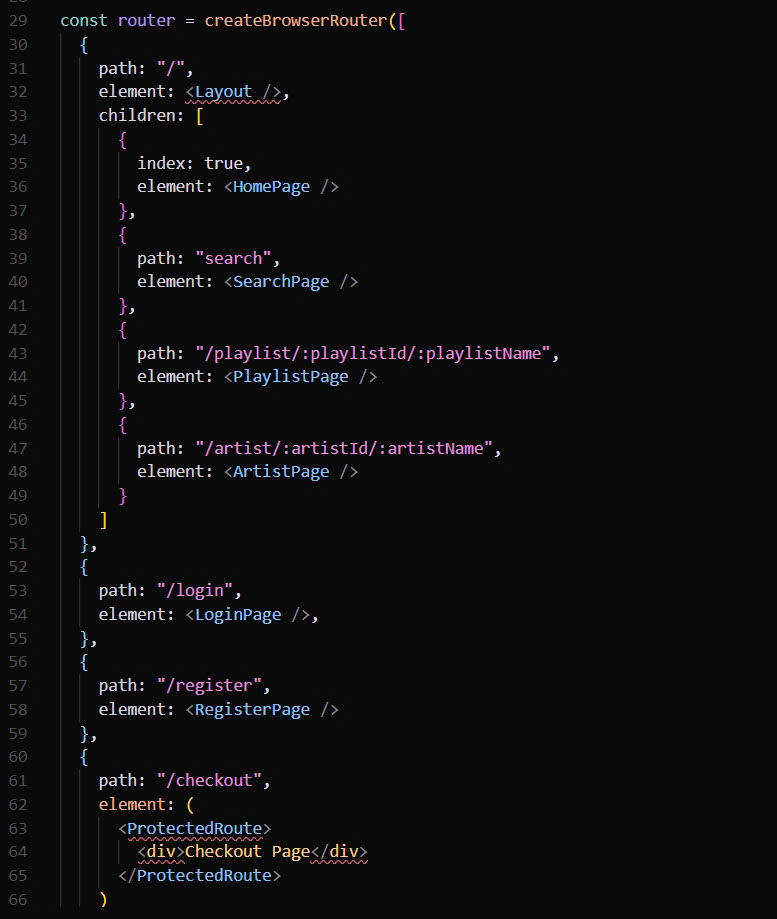
\includegraphics[width=\textwidth]{img/router1.jpg}
  \end{minipage}
  \hfill
  \begin{minipage}[b]{0.45\textwidth}
    \centering
    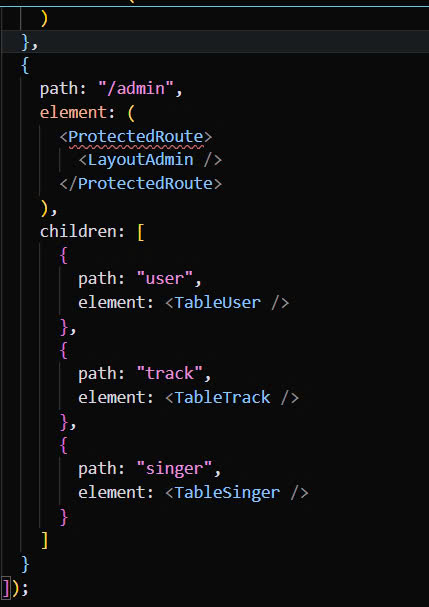
\includegraphics[width=\textwidth]{img/router2.jpg}
  \end{minipage}
\end{figure}

\textbf{Phân chia module}

\begin{itemize}
    \item pages/:
    \\ Chứa các module trang chính, mỗi trang là một module riêng biệt, ví dụ:
    \item client/ (trang cho người dùng): home, search, playlist, artist, login, register...
    \item admin/ (trang quản trị): user, track, singer...
    \\
    \item components/: Chứa các thành phần giao diện tái sử dụng, chia nhỏ theo chức năng:
    \\
    \\ layout/: Các layout tổng thể (header, sidebar, playbar, ...).
    \\
    \\ auth/: Các component liên quan xác thực, bảo vệ route.
    \\
    \\ admin/: Các component phục vụ riêng cho giao diện quản trị.
    \\
    \item services/:  Tập trung toàn bộ logic giao tiếp với API, cấu hình axios, giúp tách biệt phần giao diện và xử lý dữ liệu.
    \item context/:  Quản lý state toàn cục (người dùng, player, album...) thông qua React Context.
\end{itemize}
\\ \textbf{Một số lợi ích:}\\
Routing được tổ chức rõ ràng, tách biệt giữa các nhóm chức năng (user, admin, auth).
\\
Module được chia nhỏ theo từng chức năng, giúp dễ bảo trì, mở rộng, kiểm thử và tối ưu hiệu suất.
\\
Bảo vệ truy cập được thực hiện chặt chẽ qua ProtectedRoute.
\newpage
\section{NHIỆM VỤ VÀ VAI TRÒ THÀNH VIÊN}

\begin{table}[h]
    \centering
    \begin{tabular}{|c|c|c|} \hline 
         MSSV&  HỌ VÀ TÊN& NHIỆM VỤ\\ \hline 
         3121410237&  CAO HUY HƯNG& Backend\\ \hline 
         3121410445&  BÙI CÔNG THẠCH& Frontend\\ \hline
 3121410553& BÙI CÔNG TUẤN&Latex,  Database, Quản lý Role\\\hline
    \end{tabular}
    \label{tab:my_label}
\end{table}
\newpage

%%%%%%%%%%%%%%%%%%%%%%%%%%%%%%%%%%%%%%%%%%%%%%
 \section{KẾT QUẢ ĐẠT ĐƯỢC}
    \subsection{Màn hình trang Home}
        \begin{figure}[H]
            \centering
            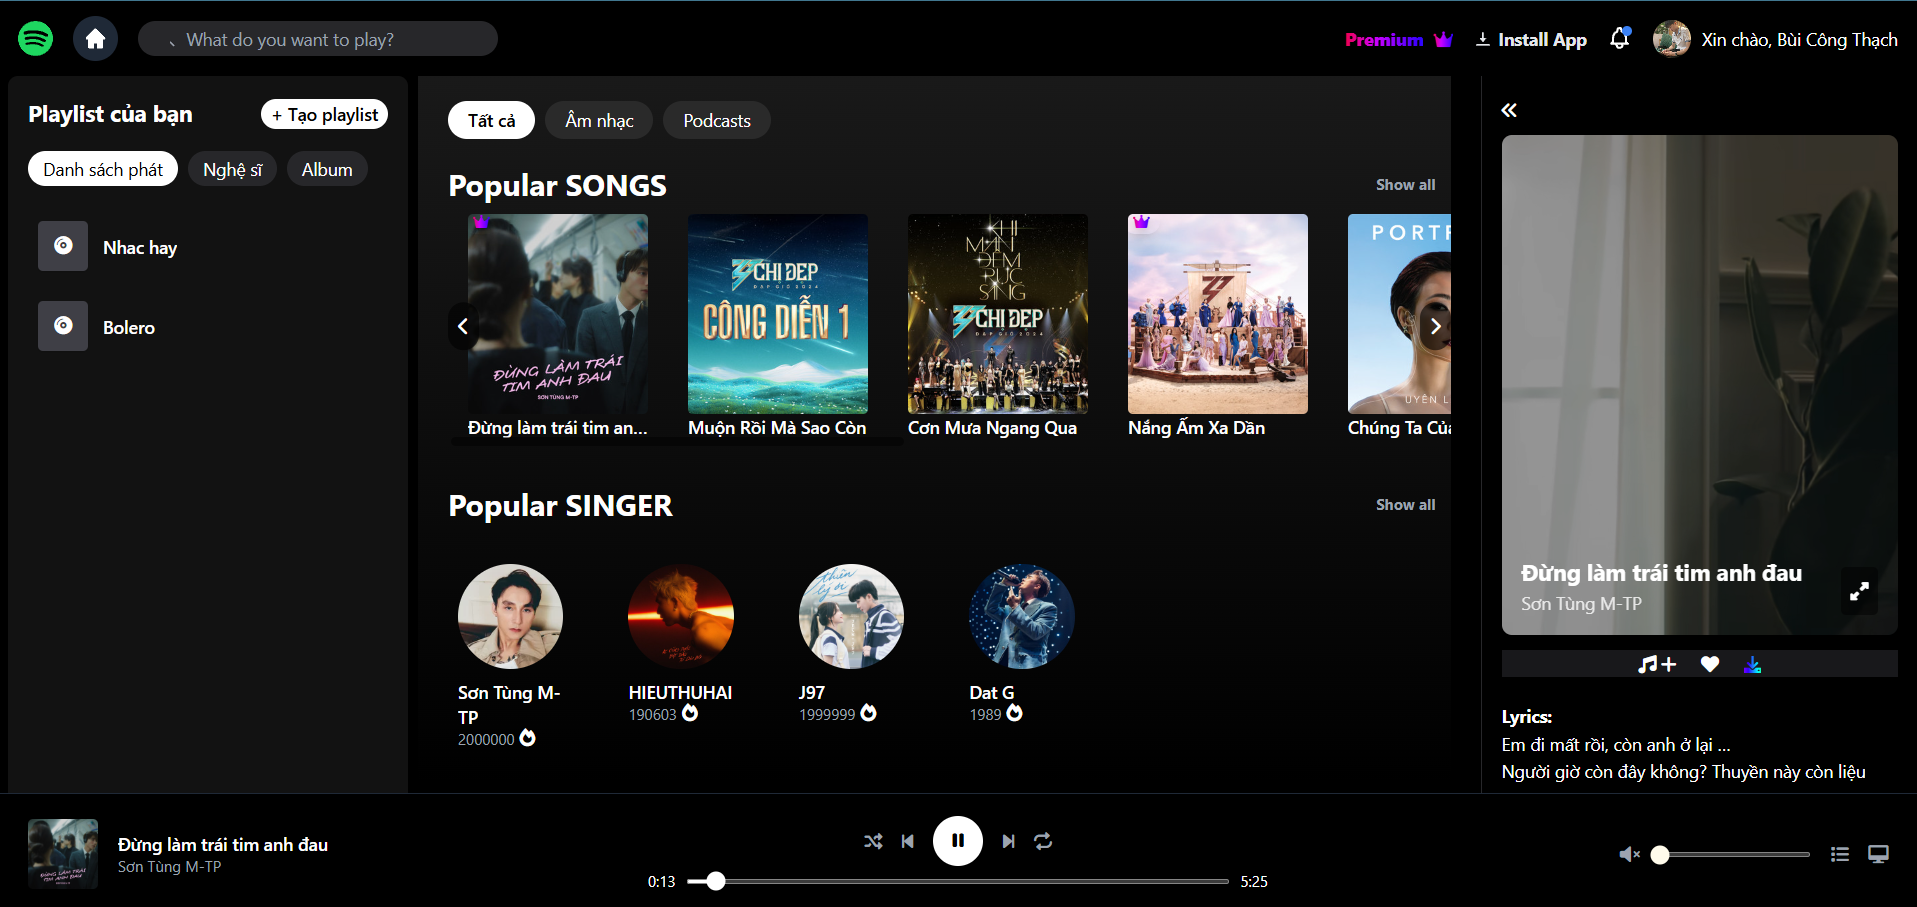
\includegraphics[width=1\linewidth]{img/homeDemo.png}
            \caption{HomePage}
            \label{fig:enter-label}
        \end{figure}
   \subsection{Màn hình Đăng nhập/Đăng ký}
   \begin{figure}[H]
       \centering
       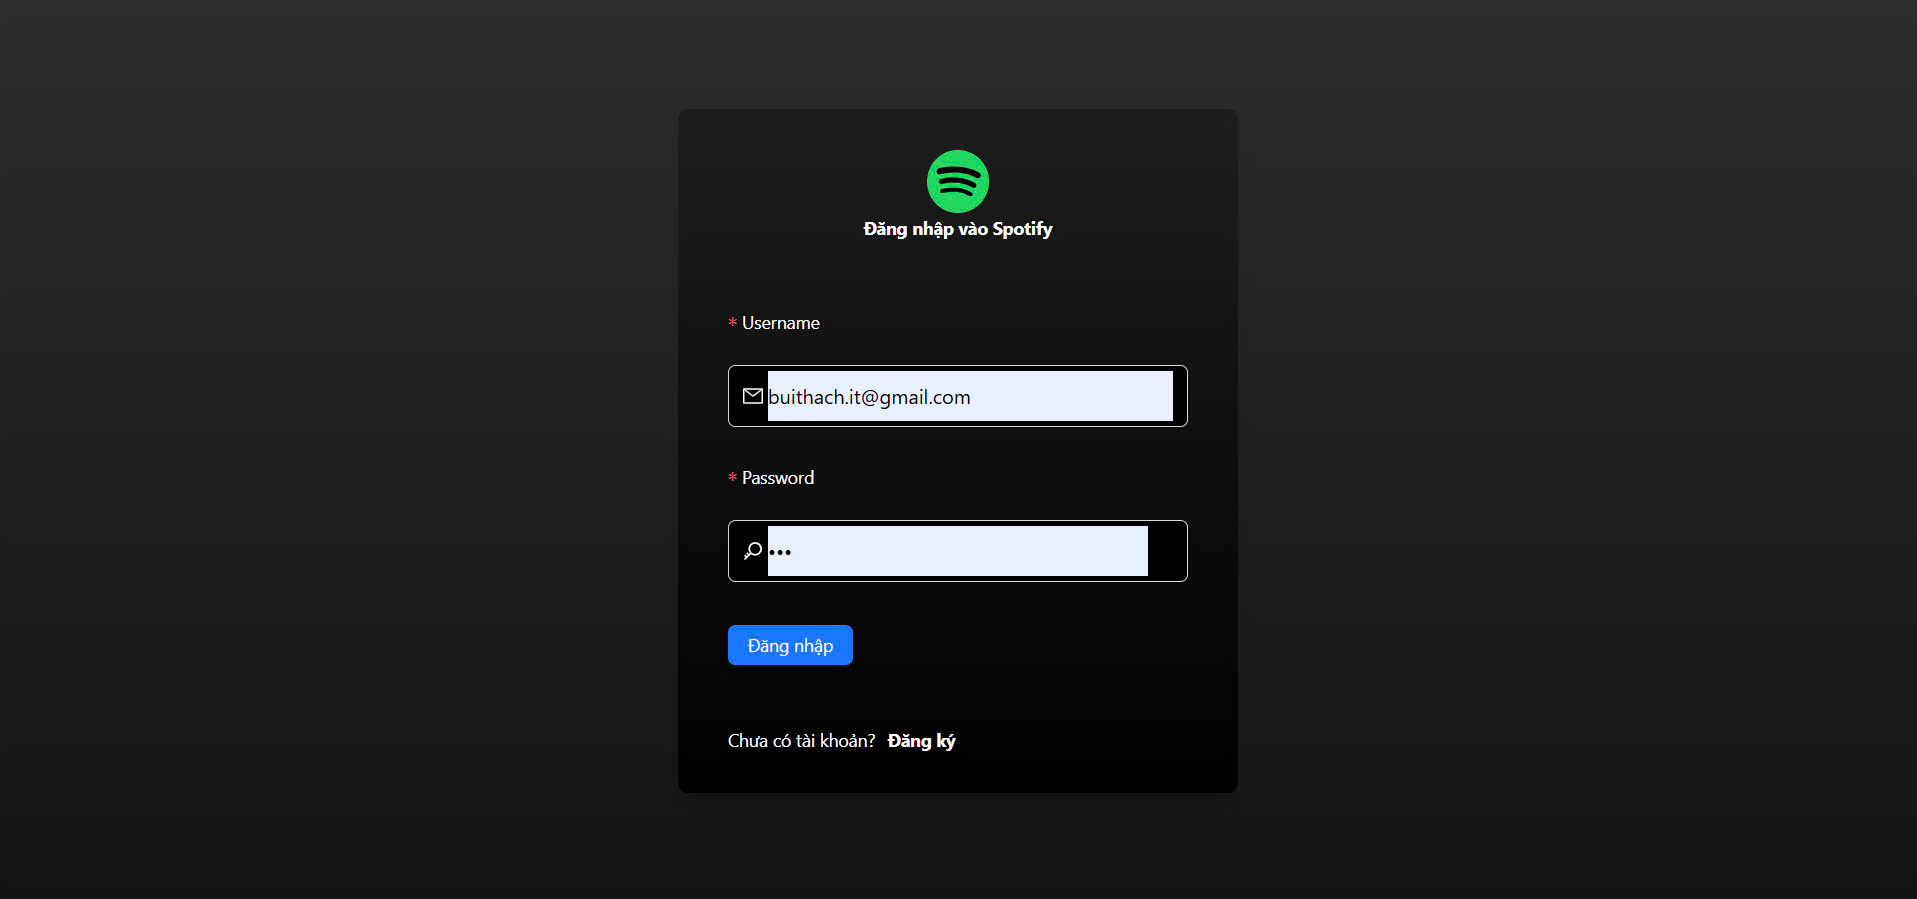
\includegraphics[width=1\linewidth]{img/login.jpg}
       \caption{Đăng nhập}
       \label{fig:enter-label}
   \end{figure}
   \begin{figure}[H]
  \centering
  \begin{minipage}[b]{1\textwidth}
    \centering
    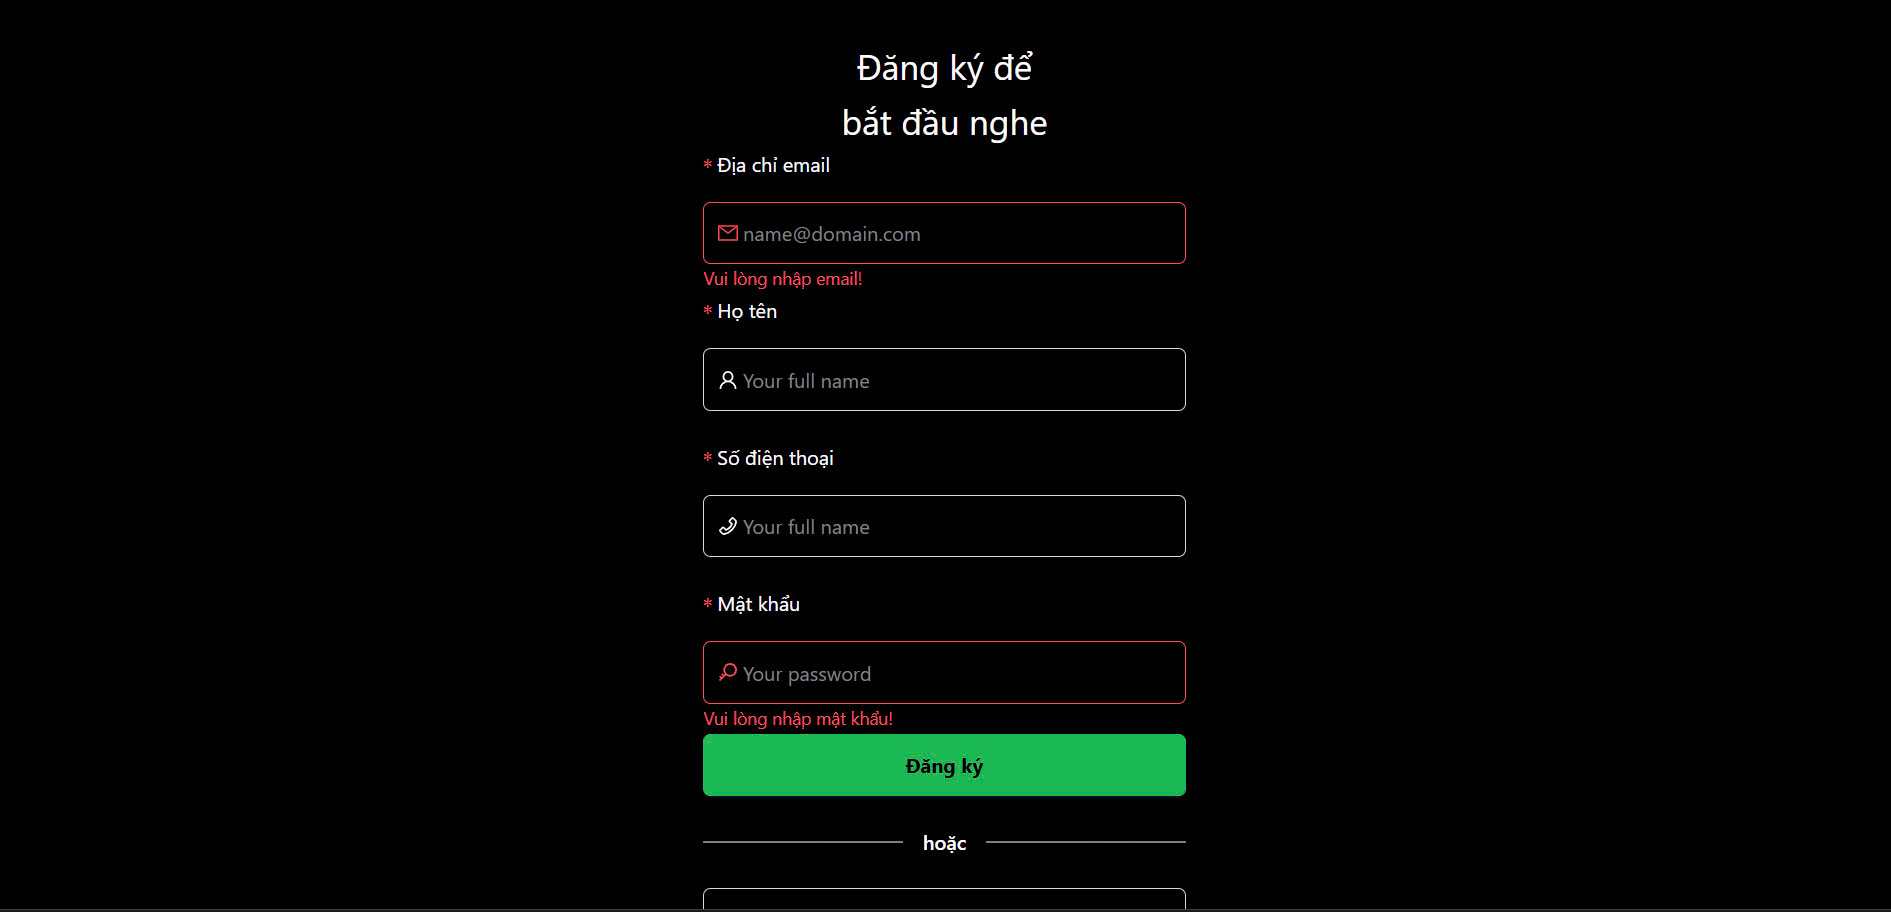
\includegraphics[width=\textwidth]{img/register1.jpg}
  \end{minipage}
  \hfill
  \begin{minipage}[b]{1\textwidth}
    \centering
    
\includegraphics[width=\textwidth]{img/register2.jpg}
  \end{minipage}
  \caption{Đăng ký}
\end{figure}

\subsection{Artist component}
\begin{figure}[H]
    \centering
    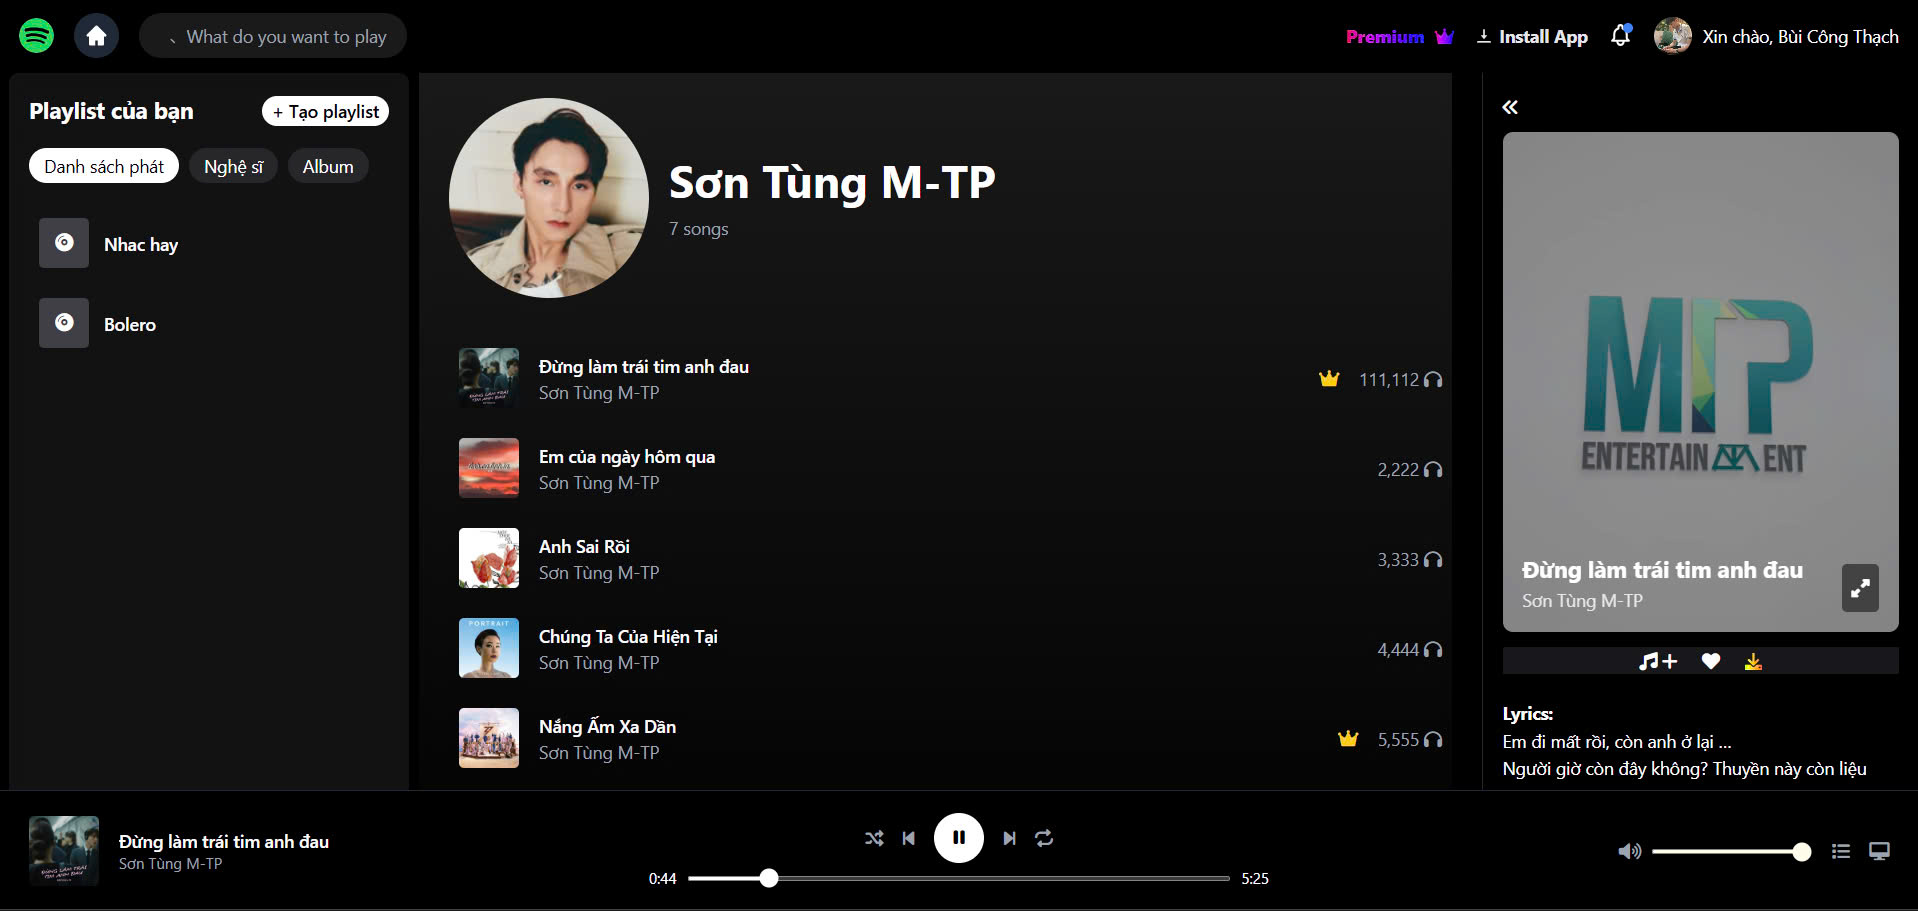
\includegraphics[width=1\linewidth]{img/artist.jpg}
    \caption{Artist component}
    \label{fig:enter-label}
\end{figure}

\subsection{Search component}
\begin{figure}[H]
    \centering
    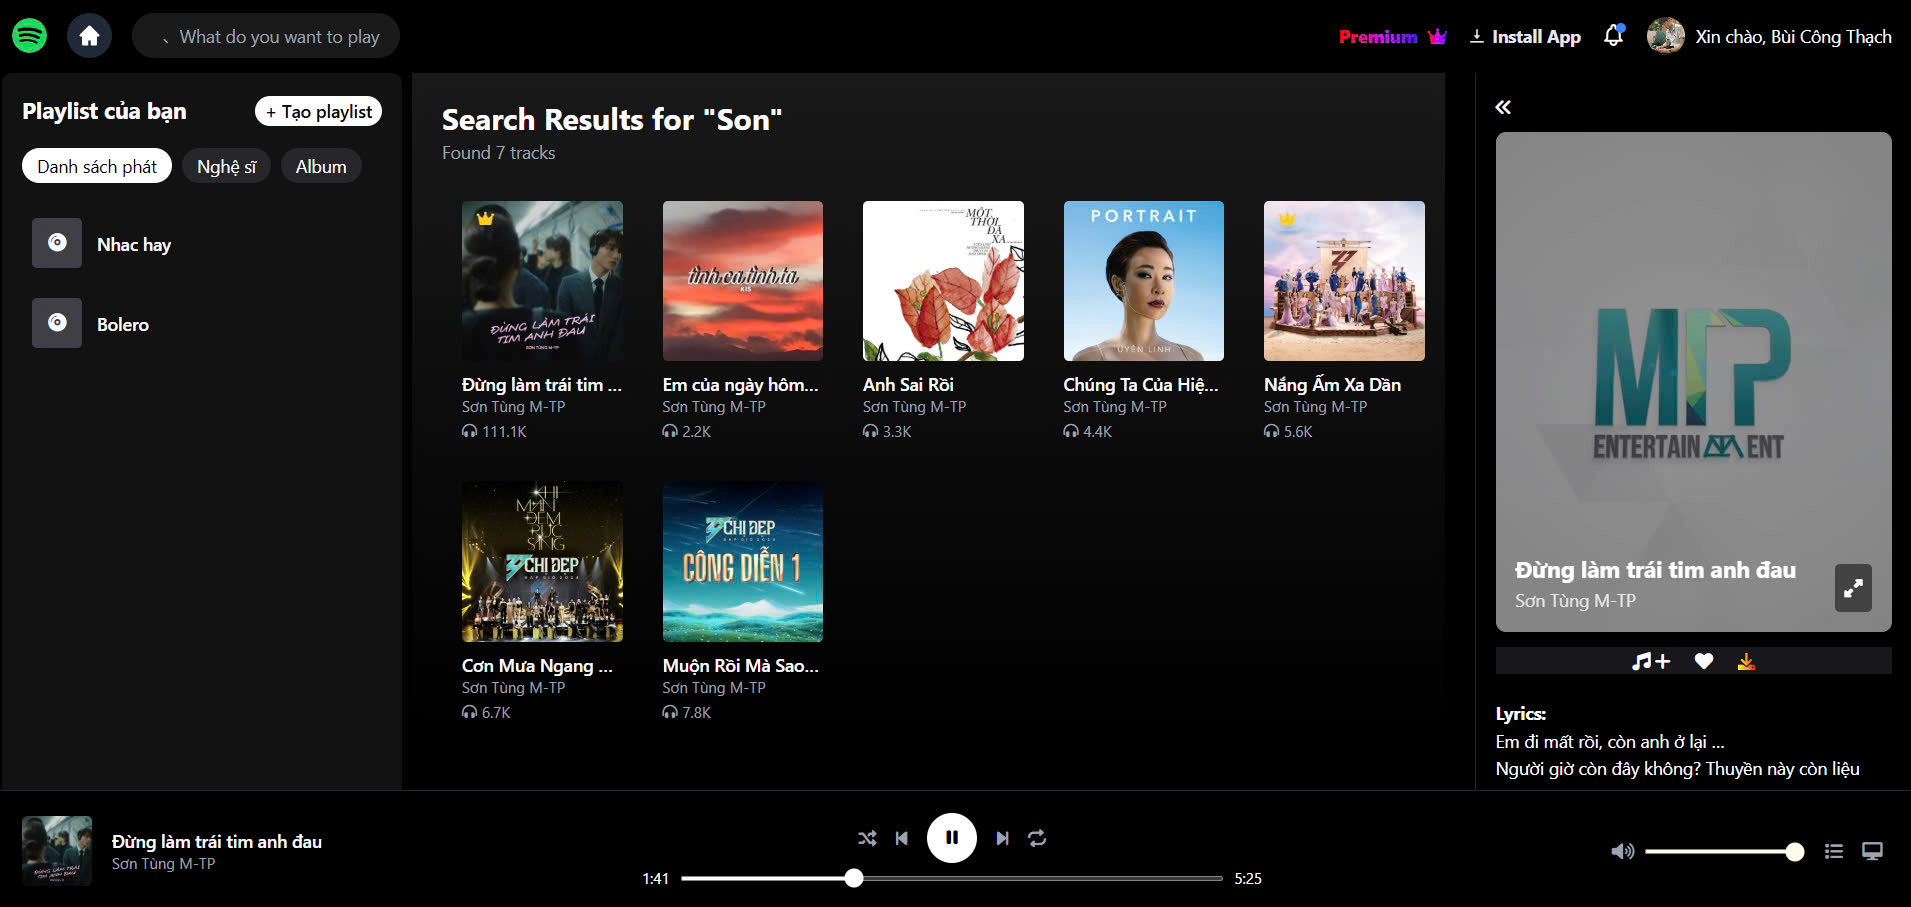
\includegraphics[width=1\linewidth]{img/search.jpg}
    \caption{Search component}
    \label{fig:enter-label}
\end{figure}

\subsection{Modal premium}
\begin{figure}[H]
    \centering
    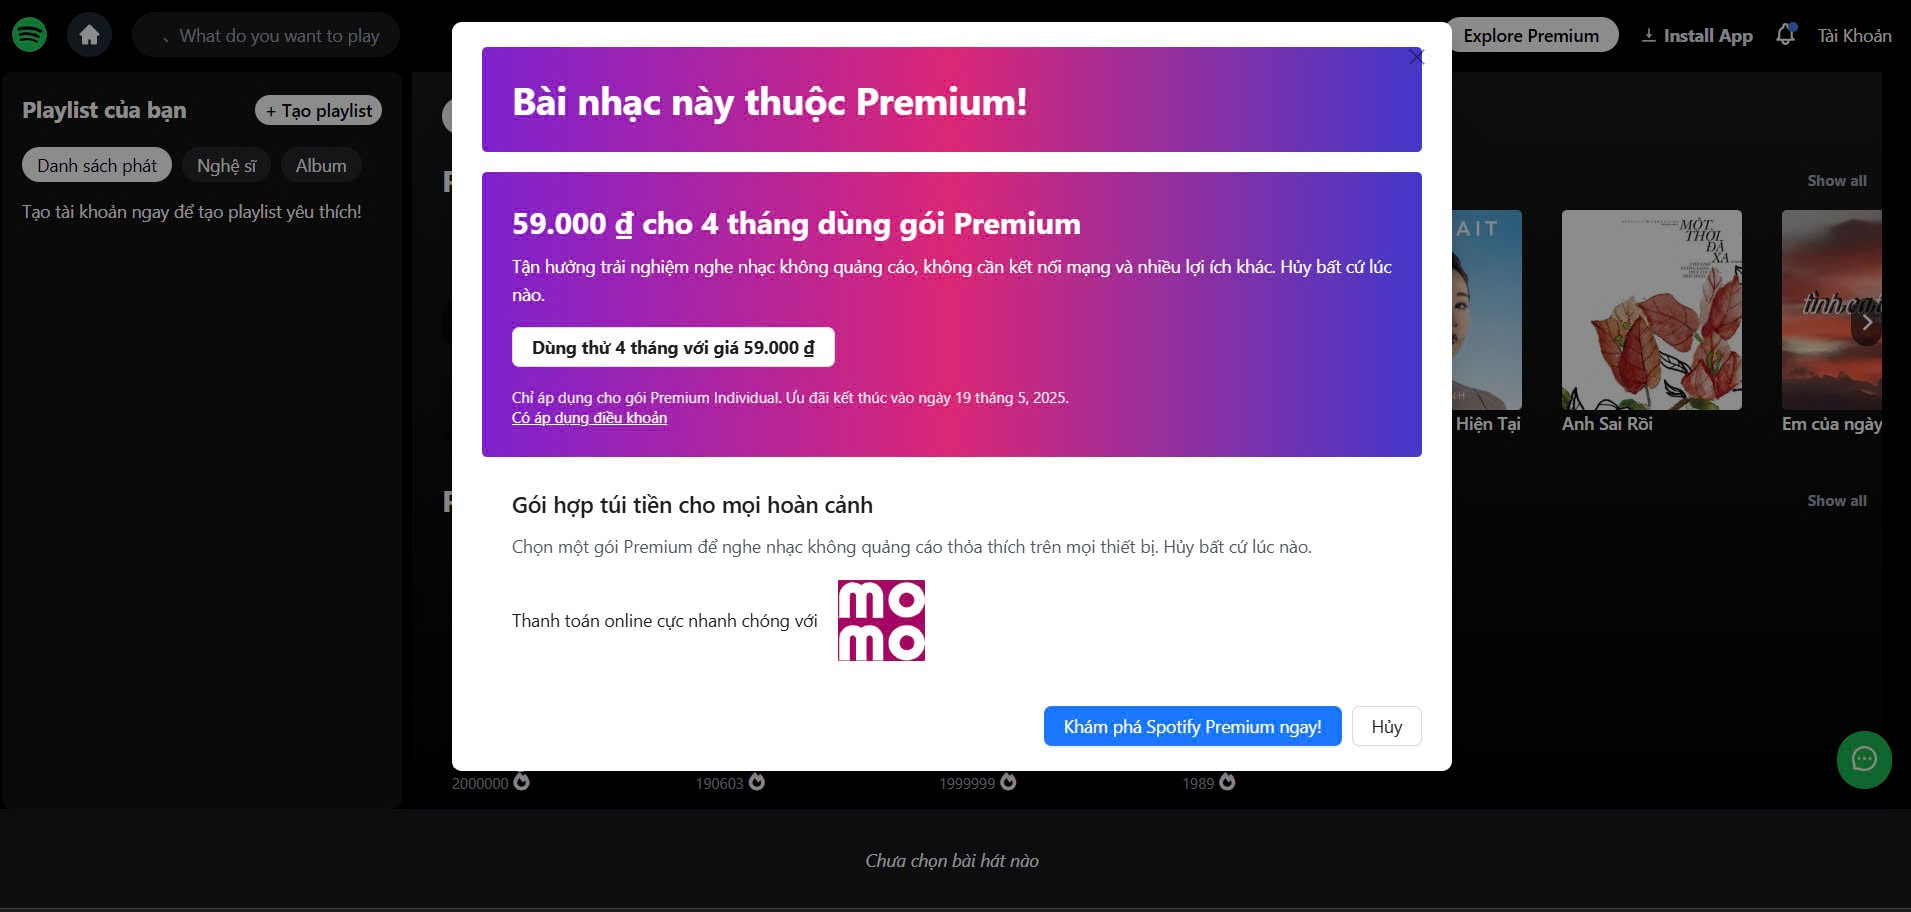
\includegraphics[width=1\linewidth]{img/payPremium.png}
    \caption{Mua Premium}
    \label{fig:enter-label}
\end{figure}

\subsection{Quản lý Người dùng}
\begin{figure}[H]
    \centering
    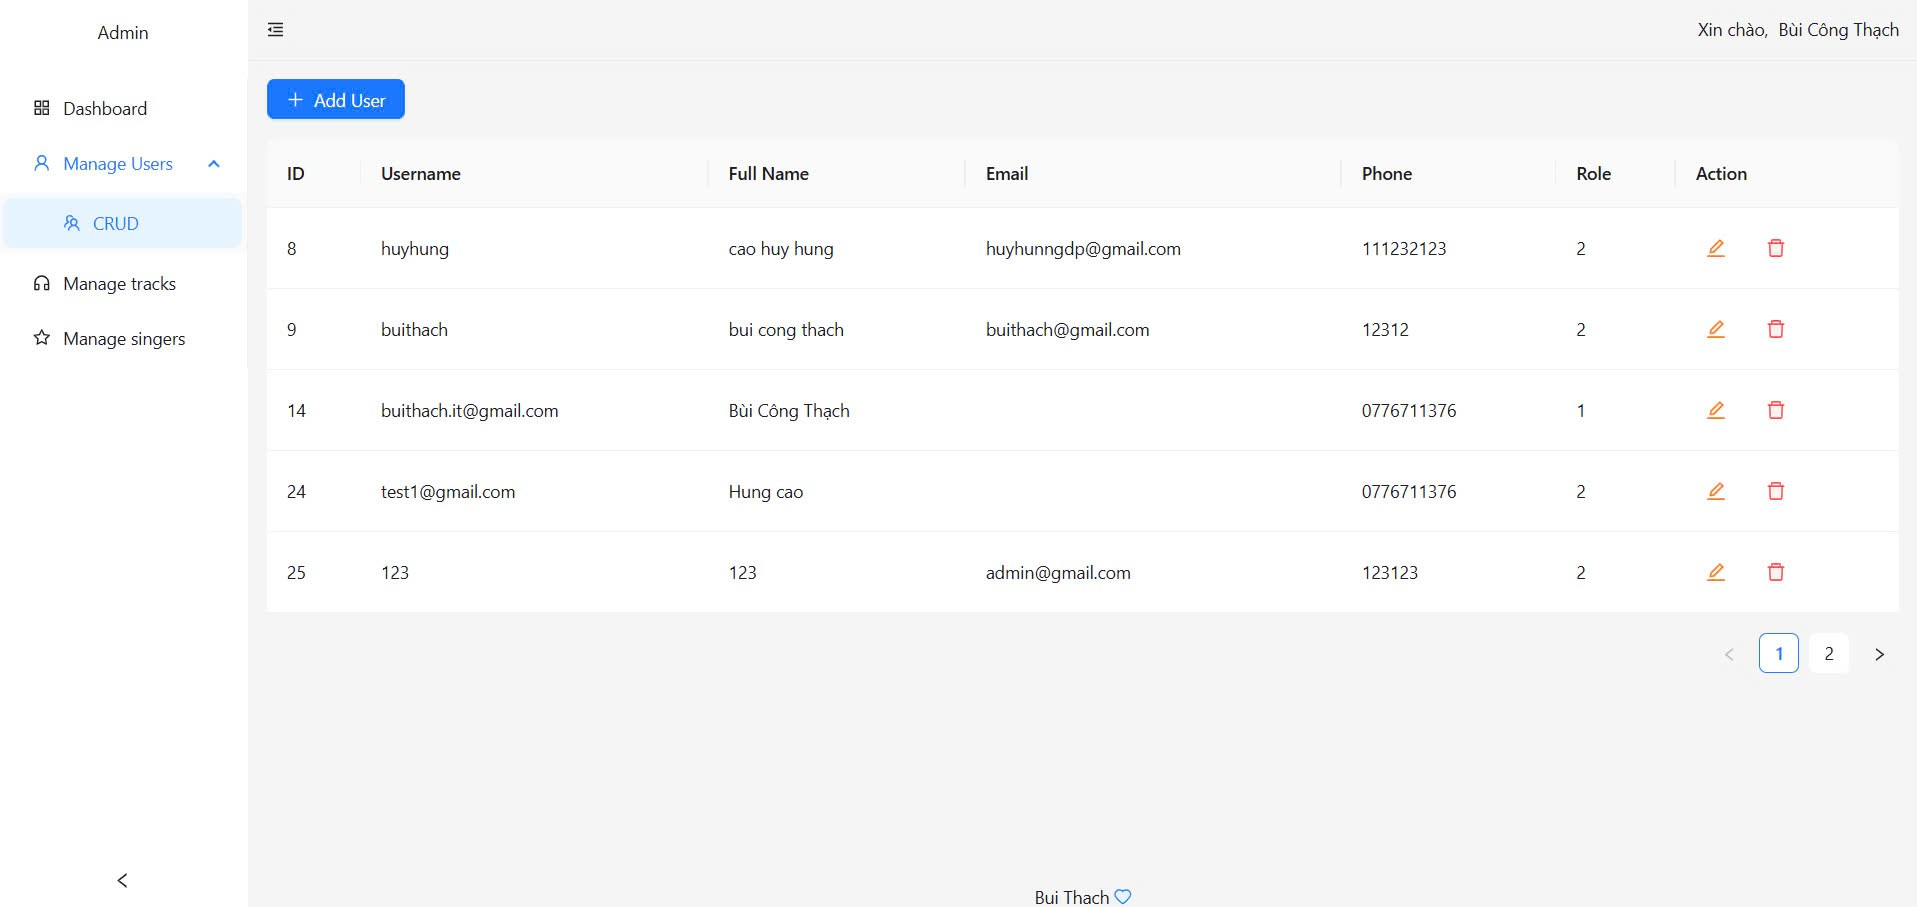
\includegraphics[width=1\linewidth]{img/User.png}
    \caption{Manage user component}
    \label{fig:enter-label}
\end{figure}

\subsection{Quản lý bài hát}
\begin{figure}[H]
    \centering
    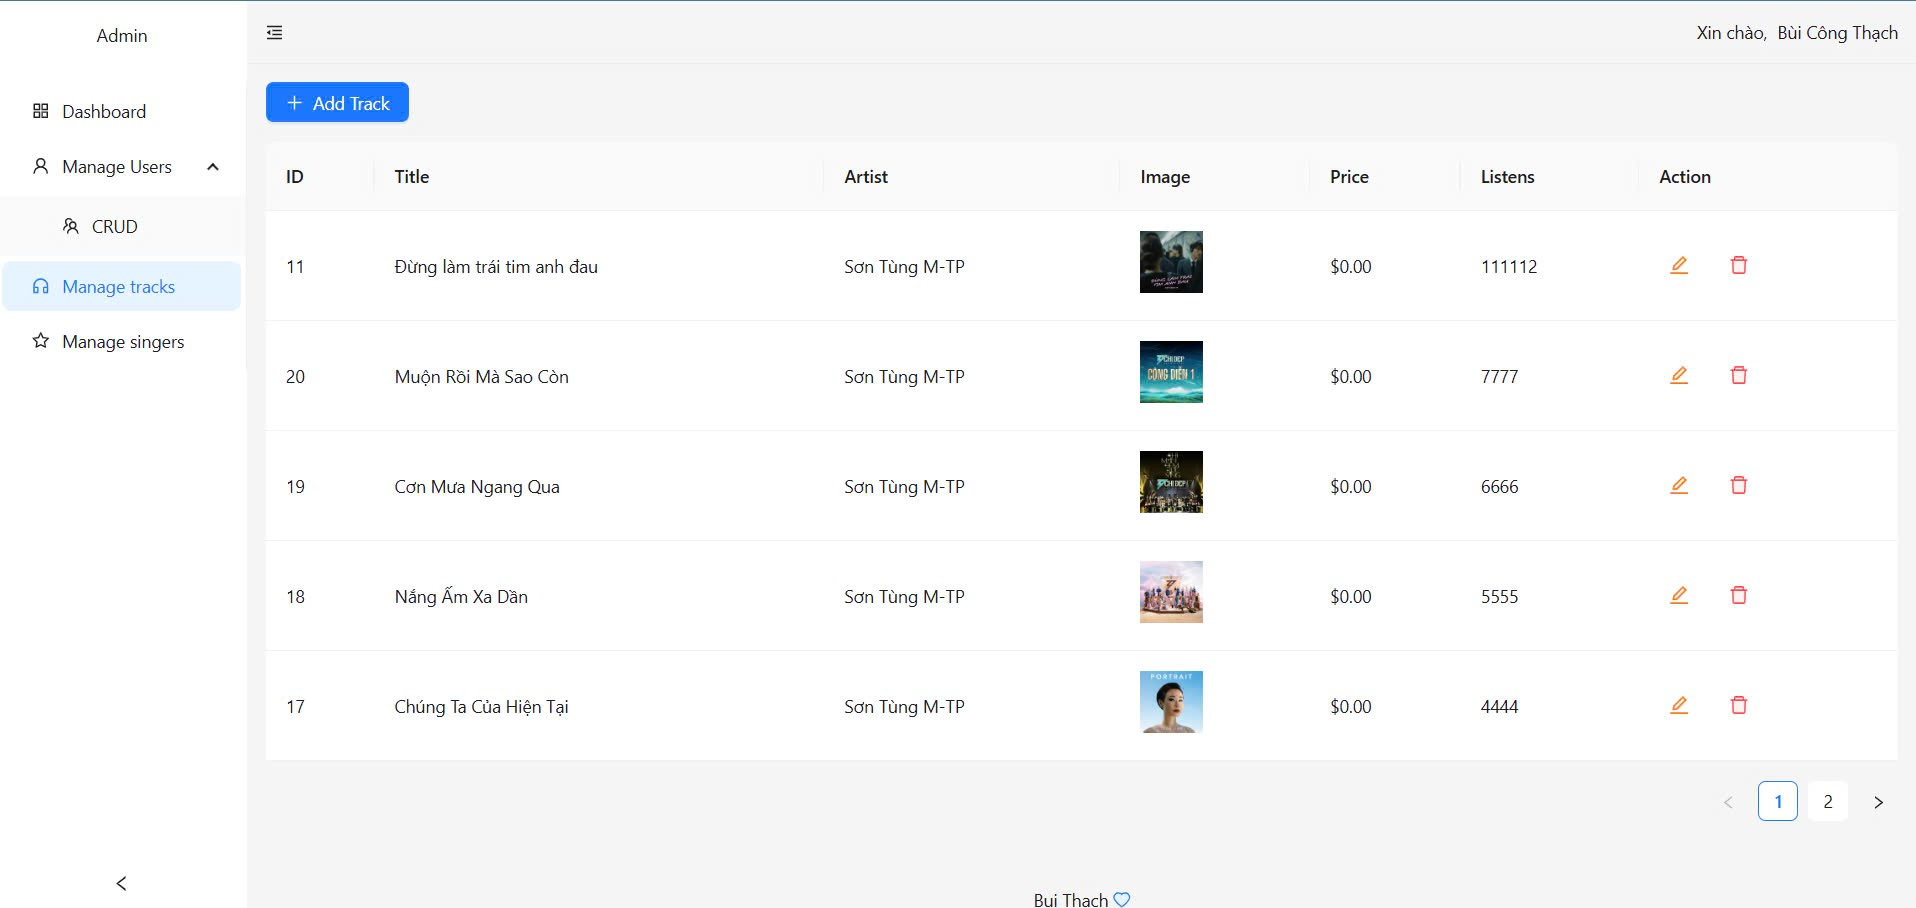
\includegraphics[width=1\linewidth]{img/tracks.png}
    \caption{Manage track component}
    \label{fig:enter-label}
\end{figure}

\subsection{Quản lý ca sĩ}
\begin{figure}[H]
    \centering
    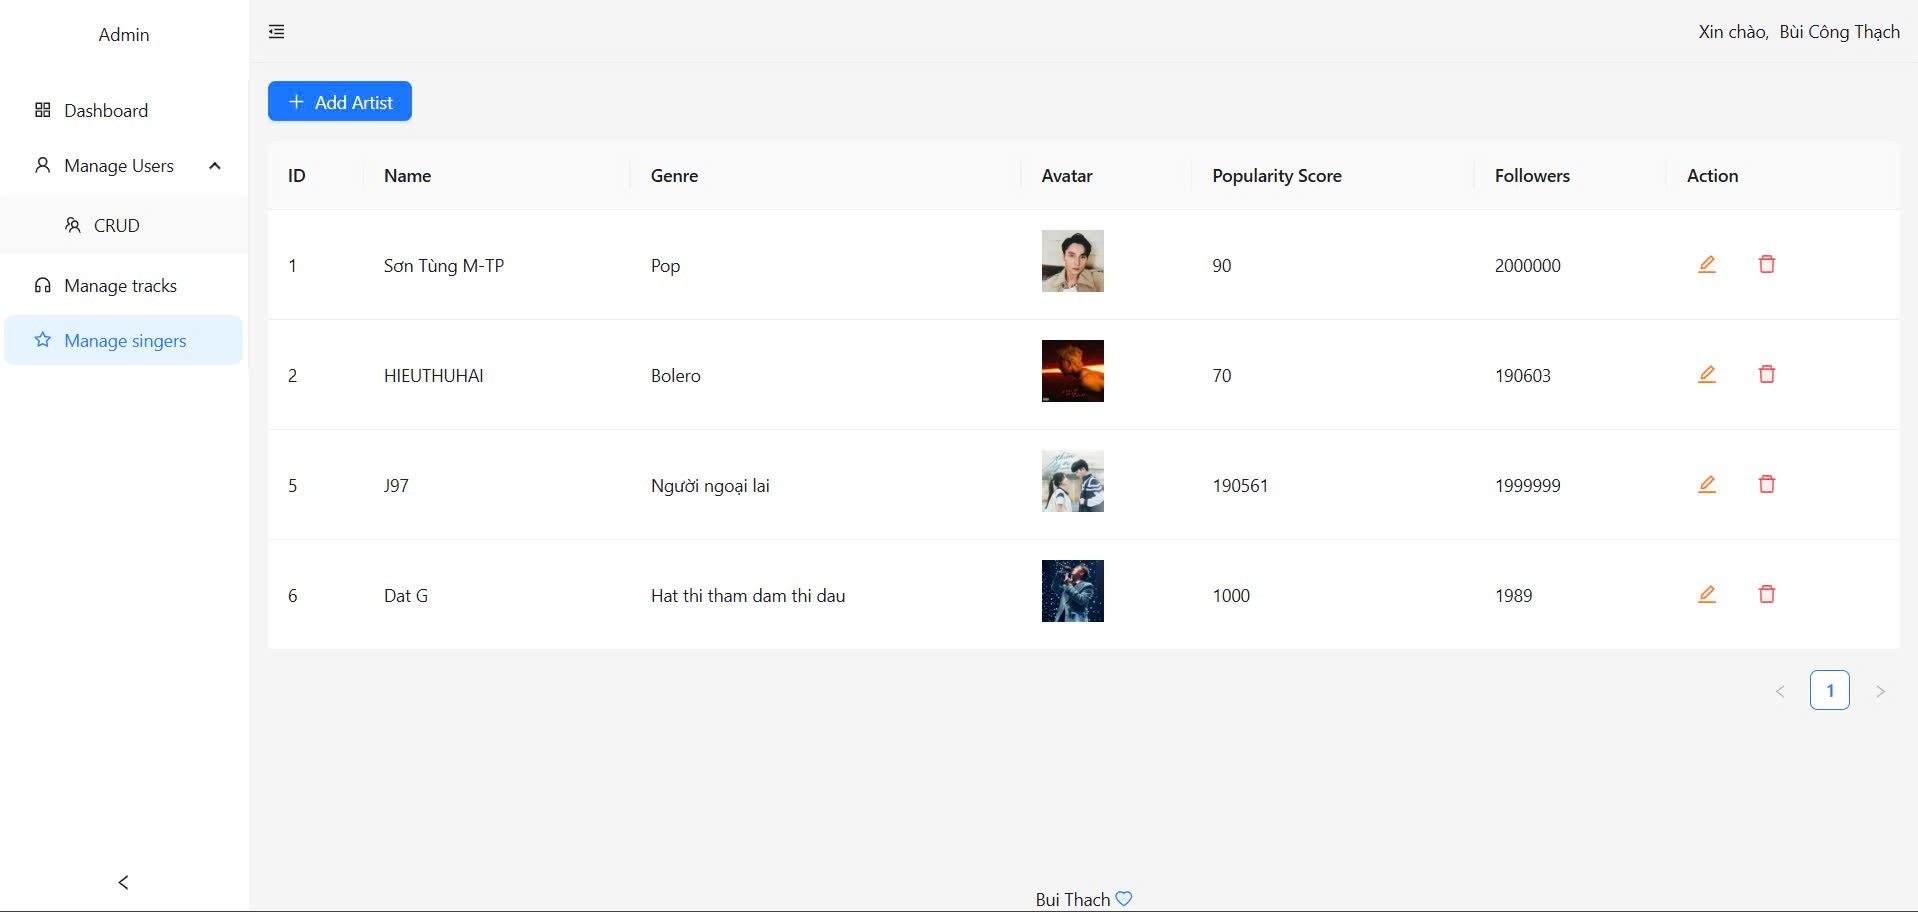
\includegraphics[width=1\linewidth]{img/singer.png}
    \caption{Manage singer component}
    \label{fig:enter-label}
\end{figure}

\subsection{AI chat}
\begin{figure}[H]
    \centering
    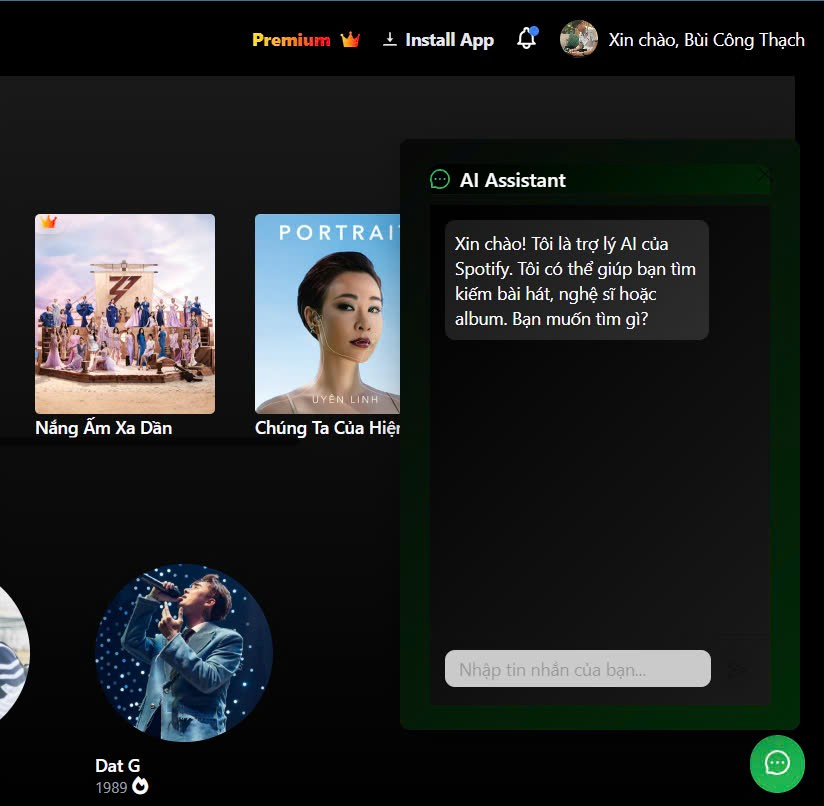
\includegraphics[width=0.6\linewidth]{img/AIchatbox.png}
    \caption{AI chatbox}
    \label{fig:enter-label}
\end{figure}

\newpage
%%%%%%%%%%%%%%%%%%%%%%%%%%%%%%%%%
\begin{thebibliography}{80}

\bibitem{LLM}
What is a large language model (LLM)?
\textbf{link: https://aws.amazon.com/vi/what-is/large-language-model/}
\bibitem{API}
Gemini 2.0 Flash
\textbf{link: https://apidog.com/vi/blog/google-gemini-2-0-api-vi/}

\end{thebibliography}
\end{document}

